\graphicspath{{./fourth/img}}

\section*{\LARGE{Введение}}
\addcontentsline{toc}{section}{Введение}
Создать примеры реализующие различные способы разметки экрана: 
\begin{itemize}
	\item Контейнер LinearLayout. Вес элемента. Программное создание 
		LinearLayout. Атрибут Layout\_gravity;
	\item Контейнер RelativeLayout. Программное создание RelativeLayout;
	\item Контейнер TableLayout. Элемент TableRow. Атрибут layout\_span. 
		Программное создание TableLayout;
	\item Контейнер FrameLayout. Атрибут android:layout\_gravity. 
		Программное создание FrameLayout в коде MainActivity;
	\item Контейнер GridLayout. Атрибуты android:rowCount и 
		android:columnCount. Атрибуты android:layout\_column,
		android:layout\_row, android:layout\_columnSpan,
		android:layout\_rowSpan.
		Программное создание GridLayout. Класс GridLayout.LayoutParams.
		Свойство columnSpec, rowSpec, leftMargin, rightMargin, topMargin,
		bottomMargin, width, height. Объект GridLayout.Spec;
	\item Контейнер ScrollView. Создание ScrollView программно в коде 
		MainActivity;
	\item Вложенные layout. Элемент include;
	\item Атрибут Gravity. Позиционирование внутри элемента. 
		Программная установка gravity.
\end{itemize}

\clearpage

\section*{\LARGE{Выполнение практической работы}}
\addcontentsline{toc}{section}{Выполнение практической работы}

\begin{image}
	%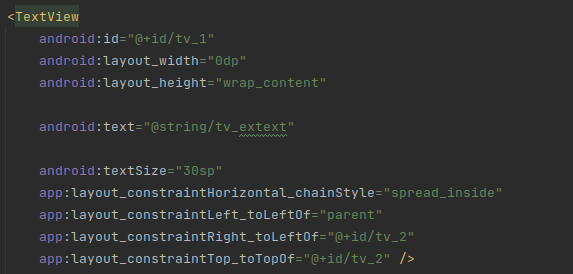
\includegraphics[width=0.9\textwidth]{Screenshot from 2023-03-28 15-20-22}
	\caption{Использование ресурсов строк в XML-коде}
	\label{fig:xml:string}
\end{image}

\section{Контейнер LinearLayout}
Контейнер LinearLayout представляет простейший контейнер - объект 
ViewGroup, который упорядочивает все дочерние элементы в одном 
направлении: по горизонтали или по вертикали. Все элементы расположены 
один за другим. Направление разметки указывается с помощью атрибута 
\texttt{android:orientation}.\par
LinearLayout поддерживает такое свойство, как вес элемента, которое 
передается атрибутом \texttt{android:layout\_weight}. Это свойство принимает 
значение, указывающее, какую часть оставшегося свободного места 
контейнера по отношению к другим объектам займет данный элемент.
Атрибут \texttt{layout\_gravity} позволяет устанавливать позиционирование 
относительно LinearLayout. Он принимает следуюшие значения:

\begin{itemize}
	\item top: выравнивает элемент по верхней границе контейнера;
	\item bottom: выравнивает элемент по нижней границе контейнера;
	\item left: выравнивает элемент по левой границе контейнера;
	\item right: выравнивает элемент по правой границе контейнера;
	\item center\_vertical: выравнивает элемент по центру по вертикали;
	\item center\_horizontal: выравнивает элемент по центру по горизонтали;
	\item center: элемент позиционируется в центре;
	\item fill\_vertical: элемент растягивается по вертикали;
	\item fill\_horizontal: элемент растягивается по горизонтали;
	\item fill: элемент заполняет все пространство контейнера;
	\item clip\_vertical: обрезает верхнюю и нижнюю границу элемента;
	\item clip\_horizontal: обрезает правую и левую границу элемента;
	\item start: элемент позиционируется в начале (в верхнем левом углу) 
		контейнера;
	\item end: элемент позиционируется в конце контейнера (в верхнем 
		правом углу).
\end{itemize}

Пример использования показан на листнинге~\ref{LinearLayout}.

\begin{lstlisting}[language=Java
	, caption=\leftline{Программное создание LinearLayout}
	, label=LinearLayout
	]
LinearLayout linearLayout = new LinearLayout(this);
linearLayout.setOrientation(LinearLayout.VERTICAL);
linearLayout.setPadding(15,30,15,30);
linearLayout.setWeightSum(4);

LinearLayout.LayoutParams layoutParams = new LinearLayout.LayoutParams(
		ViewGroup.LayoutParams.MATCH\_PARENT
		, ViewGroup.LayoutParams.WRAP\_CONTENT
		, 2
	);

TextView textView1 = new TextView(this);
textView1.setLayoutParams(layoutParams);
textView1.setText("messege 1")
textView1.setGravity(Gravity.RIGHT);
textView1.setTextSize(25);
linearLayout.addView(textView1);

TextView textView = new TextView(this);
textView.setText("messege 2");
textView.setBackgroundResource(R.color.teal\_200);
textView.setTextSize(30);
textView.setLayoutParams(layoutParams);
linearLayout.addView(textView);

TextView textView2 = new TextView(this);
textView2.setLayoutParams(layoutParams);
textView2.setHint("messege 3");
textView2.setGravity(Gravity.CENTER\_HORIZONTAL);
textView2.setTextSize(45);
linearLayout.addView(textView2);
\end{lstlisting}

\section{Контейнер RelativeLayout}
RelativeLayout представляет объект ViewGroup, который располагает 
дочерние элементы относительно позиции других дочерних элементов 
разметки или относительно области самой разметки RelativeLayout. 
Используя относительное позиционирование, мы можем установить элемент 
по правому краю или в центре или иным способом, который предоставляет 
данный контейнер. Для установки элемента в файле xml предоставляет 
данный контейнер. Для установки элемента в файле xml мы можем 
применять следующие атрибуты:

\begin{itemize}
	\item \texttt{android:layout\_above}: располагает элемент над
		элементом с указанным Id;
	\item \texttt{android:layout\_below:} располагает элемент под
		элементом с указанным Id;
	\item \texttt{android:layout\_toLeftOf}: располагается слева от
		элемента с указанным Id;
	\item \texttt{android:layout\_toRightOf}: располагается справа от
		элемента с указанным Id;
	\item \texttt{android:layout\_toStartOf}: располагает начало текущего
		элемента, где начинается элемент с указанным Id;
	\item \texttt{android:layout\_toEndOf}: располагает начало текущего
		элемента, где завершается элемент с указанным Id;
	\item \texttt{android:layout\_alignBottom}: выравнивает элемент по
		нижней границе другого элемента с указанным Id;
	\item \texttt{android:layout\_alignLeft}: выравнивает элемент по
		левой границе другого элемента с указанным Id;
	\item \texttt{android:layout\_alignRight}: выравнивает элемент по
		правой границе другого элемента с указанным Id;
	\item \texttt{android:layout\_alignStart}: выравнивает элемент по линии,
		у которой начинается другой элемент с указанным Id;
	\item \texttt{android:layout\_alignEnd}: выравнивает элемент по линии,
		у которой завершается другой элемент с указанным Id;
	\item \texttt{android:layout\_alignTop}: выравнивает элемент по верхней
		границе другого элемента с указанным Id;
	\item \texttt{android:layout\_alignBaseline}: выравнивает базовую линию
		элемента по базовой линии другого элемента с указанным Id;
	\item \texttt{android:layout\_alignParentBottom}: если атрибут имеет
		значение true, то элемент прижимается к нижней границе контейнера;
	\item \texttt{android:layout\_alignParentRight}: если атрибут имеет
		значение true, то элемент прижимается к правому краю контейнера;
	\item \texttt{android:layout\_alignParentLeft}: если атрибут имеет
		значение true, то элемент прижимается к левому краю контейнера;
	\item \texttt{android:layout\_alignParentStart}: если атрибут имеет
		значение true, то элемент прижимается к начальному краю контейнера
		(при левосторонней ориентации текста - левый край);
	\item \texttt{android:layout\_alignParentEnd}: если атрибут имеет значение
		true, то элемент прижимается к конечному краю контейнера
		(при левосторонней ориентации текста - правый край);
	\item \texttt{android:layout\_alignParentTop}: если атрибут имеет значение
		true, то элемент прижимается к верхней границе контейнера;
	\item \texttt{android:layout\_centerInParent}: если атрибут имеет значение
		true, то элемент располагается по центру родительского контейнера;
	\item \texttt{android:layout\_centerHorizontal}: при значении true
		выравнивает элемент по центру по горизонтали;
	\item \texttt{android:layout\_centerVertical}: при значении true
		выравнивает элемент по центру по вертикали.
\end{itemize}

Пример использования показан на листнинге~\ref{RelativeLayout}.

\begin{lstlisting}[language=Java
	, caption=\leftline{Программное создание RelativeLayout}
	, label=RelativeLayout
	]
RelativeLayout relativeLayout = new RelativeLayout(this);
relativeLayout.setPadding(20,20,20,20);
TextView textView1 = new TextView(this);
textView1.setText("left up");
textView1.setTextSize(getResources().getDimension(R.dimen.textSize));
TextView textView2 = new TextView(this);
textView2.setText("right up");
textView2.setTextSize(getResources().getDimension(R.dimen.textSize));
TextView textView3 = new TextView(this);
textView3.setText("left down");
textView3.setTextSize(getResources().getDimension(R.dimen.textSize));
TextView textView4 = new TextView(this);
textView4.setText("right down");
textView4.setTextSize(getResources().getDimension(R.dimen.textSize));

RelativeLayout.LayoutParams layoutParams1 = new RelativeLayout.LayoutParams(ViewGroup.LayoutParams.WRAP\_CONTENT, ViewGroup.LayoutParams.WRAP\_CONTENT);
layoutParams1.addRule(RelativeLayout.ALIGN\_PARENT\_LEFT);
layoutParams1.addRule(RelativeLayout.ALIGN\_PARENT\_TOP);
relativeLayout.addView(textView1, layoutParams1);

RelativeLayout.LayoutParams layoutParams2 = new RelativeLayout.LayoutParams(ViewGroup.LayoutParams.WRAP\_CONTENT, ViewGroup.LayoutParams.WRAP\_CONTENT);
layoutParams2.addRule(RelativeLayout.ALIGN\_PARENT\_RIGHT);
layoutParams2.addRule(RelativeLayout.ALIGN\_PARENT\_TOP);
relativeLayout.addView(textView2, layoutParams2);

RelativeLayout.LayoutParams layoutParams3 = new RelativeLayout.LayoutParams(ViewGroup.LayoutParams.WRAP\_CONTENT, ViewGroup.LayoutParams.WRAP\_CONTENT);
layoutParams3.addRule(RelativeLayout.ALIGN\_PARENT\_LEFT);
layoutParams3.addRule(RelativeLayout.ALIGN\_PARENT\_BOTTOM);
relativeLayout.addView(textView3, layoutParams3);

RelativeLayout.LayoutParams layoutParams4 = new RelativeLayout.LayoutParams(ViewGroup.LayoutParams.WRAP\_CONTENT, ViewGroup.LayoutParams.WRAP\_CONTENT);
layoutParams4.addRule(RelativeLayout.ALIGN\_PARENT\_RIGHT);
layoutParams4.addRule(RelativeLayout.ALIGN\_PARENT\_BOTTOM);
relativeLayout.addView(textView4, layoutParams4);

setContentView(relativeLayout);
\end{lstlisting}

\section{Контейнер TableLayout}
Контейнер TableLayout структурирует элементы управления в виде 
таблицы по столбцам и строкам. Используя элемент TableRow, мы создаем 
отдельную строку. Причем элемент TableRow наследуется от класса 
LinearLayout, поэтому мы можем к нему применять тот же функционал, что и 
к LinearLayout. В частности, для определения пространства для элементов в 
строке используется атрибут \texttt{android:layout\_weight}.
Если какой-то элемент должен быть растянут на ряд столбцов, то мы можем
растянуть его с помощью атрибута \texttt{layout\_span}, который указывает
на какое количество столбцов надо растянуть элемент.

Пример использования показан на листнинге~\ref{TableLayout}.

\begin{lstlisting}[language=XML
	, caption=\leftline{Программное создание TableLayout}
	, label=TableLayout
	]
<TableLayout
android:layout_width="match_parent"
android:layout_height="match_parent">
	<TableRow>
		<TextView
			android:layout_weight="0.5"
			android:text="1"
			android:textSize="30sp"
			android:background="@color/purple_200"
			android:gravity="center"
			android:layout_width="wrap_content"
			android:layout_height="wrap_content" />
		<TextView
			android:layout_weight="0.5"
			android:text="2"
			android:textSize="30sp"
			android:gravity="center"
			android:layout_width="wrap_content"
			android:layout_height="wrap_content" />
		<TextView
			android:layout_weight="0.5"
			android:text="3"
			android:textSize="30sp"
			android:gravity="center"
			android:layout_width="wrap_content"
			android:layout_height="wrap_content" />
		<TextView
			android:layout_weight="0.5"
			android:text="4"
			android:textSize="30sp"
			android:gravity="center"
			android:background="@color/purple_200"
			android:layout_width="wrap_content"
			android:layout_height="wrap_content" />
	</TableRow>
	<TableRow>
		<TextView
			android:layout_weight="0.5"
			android:text="5"
			android:textSize="30sp"
			android:gravity="center"
			android:layout_width="wrap_content"
			android:layout_height="wrap_content" />
		<TextView
			android:layout_weight="0.5"
			android:text="6"
			android:textSize="30sp"
			android:gravity="center"
			android:layout_width="wrap_content"
			android:layout_height="wrap_content" />
		<TextView
			android:layout_weight="0.5"
			android:text="7"
			android:textSize="30sp"
			android:gravity="center"
			android:layout_width="wrap_content"
			android:layout_height="wrap_content" />
		<TextView
			android:layout_weight="0.5"
			android:text="8"
			android:textSize="30sp"
			android:gravity="center"
			android:background="@color/purple_200"
			android:layout_width="wrap_content"
			android:layout_height="wrap_content" />
		<TextView
			android:layout_weight="0.5"
			android:text="9"
			android:textSize="30sp"
			android:gravity="center"
			android:layout_width="wrap_content"
			android:layout_height="wrap_content" />
	</TableRow>
	<TableRow>
		<TextView
			android:layout_weight="0.5"
			android:text="10"
			android:textSize="30sp"
			android:gravity="center"
			android:layout_width="wrap_content"
			android:layout_height="wrap_content" />
		<TextView
			android:layout_weight="0.5"
			android:text="12"
			android:textSize="30sp"
			android:gravity="center"
			android:background="@color/purple_200"
			android:layout_width="wrap_content"
			android:layout_height="wrap_content" />
		<TextView
			android:layout_weight="0.5"
			android:text="13"
			android:textSize="30sp"
			android:gravity="center"
			android:layout_width="wrap_content"
			android:layout_height="wrap_content" />
		<TextView
			android:layout_weight="0.5"
			android:text="14"
			android:textSize="30sp"
			android:gravity="center"
			android:layout_width="wrap_content"
			android:layout_height="wrap_content" />
	</TableRow>
</TableLayout>
\end{lstlisting}

\section{Контейнер FrameLayout}
Контейнер FrameLayout предназначен для вывода на экран одного 
помещенного в него визуального элемента. Если же мы поместим несколько 
элементов, то они будут накладываться друг на друга. Тем не менее также 
можно располагать в FrameLayout несколько элементов. Элементы 
управления, которые помещаются в FrameLayout, могут установить свое 
позиционирование с помощью атрибута \texttt{android:layout\_gravity}.\par
Нередко FrameLayout применяется для создания производных контейнеров,
например, ScrollView, который обеспечивает прокрутку.

Пример использования показан на листнинге~\ref{FrameLayout}.

\begin{lstlisting}[language=XML
	, caption=\leftline{Программное создание FrameLayout}
	, label=FrameLayout
	]
<FrameLayout
    xmlns:android="http://schemas.android.com/apk/res/android"
    android:layout_width="match_parent"
    android:layout_height="match_parent">
    <TextView
        android:layout_width="wrap_content"
        android:layout_height="wrap_content"
        android:text="First message"
        android:textSize="80sp"
        android:layout_gravity="center_horizontal" />
    <TextView
        android:layout_width="wrap_content"
        android:layout_height="wrap_content"
        android:text="Second message"
        android:textSize="40sp"
        android:layout_gravity="center"/>
    <TextView
        android:layout_width="wrap_content"
        android:layout_height="wrap_content"
        android:text="Third message"
        android:textSize="50sp"
        android:layout_gravity="bottom|center_horizontal"/>
</FrameLayout>
\end{lstlisting}

\section{Контейнер GridLayout}
GridLayout представляет еще один контейнер, который позволяет 
создавать табличные представления. \texttt{GridLayout} состоит из коллекции
строк, каждая из которых состоит из отдельных ячеек. С помощью атрибутов 
\texttt{android:rowCount} и \texttt{android:columnCount} устанавливается
число строк и столбцов соответственно. При этом ширина столбцов
устанавливается автоматически по ширине самого широкого элемента. 
Однако мы можем явно задать номер столбца и строки для 
определенного элемента, а при необходимости растянуть на несколько 
столбцов или строк. Для этого мы можем применять следующие атрибуты:

\begin{itemize}
	\item \texttt{android:layout\_column}: номер столбца (отсчет идет от нуля);
	\item \texttt{android:layout\_row}: номер строки;
	\item \texttt{android:layout\_columnSpan}: количество столбцов, на которые 
		растягивается элемент;
	\item \texttt{android:layout\_rowSpan}: количество строк, на которые 
		растягивается элемент.
\end{itemize}

Класс \texttt{GridLayout.LayoutParams} имеет ряд свойств, которые позволяют 
настроить расположение: 

\begin{itemize}
	\item \texttt{columnSpec}: задает столбец для расположения
		в виде объекта \texttt{GridLayout.Spec};
	\item \texttt{rowSpec}: задает строку для расположения
		в виде объекта \texttt{GridLayout.Spec};
	\item \texttt{leftMargin}: задает отступ слева;
	\item \texttt{rightMargin}: задает отступ справа;
	\item \texttt{topMargin}: задает отступ сверху;
	\item \texttt{bottomMargin}: задает отступ снизу;
	\item \texttt{width}: задает ширину виджета;
	\item \texttt{height}: задает высоту виджета. 
\end{itemize}

Объект \texttt{GridLayout.Spec} позволяет задать размещение в ячейках 
столбца или строки. Для создание этого объекта применяется статический 
метод \texttt{GridLayout.spec()}, который имеет ряд версий.
Отметим среди них следующие:

\begin{itemize}
	\item \texttt{GridLayout.spec(int)}: задает столбец или строку,
		где располагается виджет. Отсчет ячеек начинается с нуля.
		Виджет занимает только одну ячейку;
	\item \texttt{GridLayout.spec(int, int)}: первый параметр задает столбец
		или строку, где располагается виджет. Второй параметр указывает,
		насколько ячеек растягивается виджет;
	\item \texttt{GridLayout.spec(int, android.widget.GridLayout.Alignment)}:
		первый параметр задает столбец или строку, где располагается виджет.
		Второй параметр устанавливает выравнивание виджета;
	\item \texttt{GridLayout.spec(int, int,
		android.widget.GridLayout.Alignment)}: первый параметр задает столбец
		или строку, где располагается виджет. Второй параметр указывает,
		насколько ячеек растягивается виджет. Третий параметр устанавливает
		выравнивание виджета.
\end{itemize}


Пример использования показан на листнинге~\ref{GridLayout}.

\begin{lstlisting}[language=XML
	, caption=\leftline{Программное создание GridLayout}
	, label=GridLayout
	]
<GridLayout
	xmlns:android="http://schemas.android.com/apk/res/android"
    android:layout_width="match_parent"
    android:layout_height="match_parent"
    android:rowCount="5"
    android:columnCount="5">
    <Button
        android:text="1"
        android:layout_column="0"
        android:layout_row="0" />
    <Button android:text="2"
        android:layout_column="1"
        android:layout_row="0"/>
    <Button android:text="3"
        android:layout_column="2"
        android:layout_row="0" />
    <Button android:text="4"
        android:layout_width="180dp"
        android:layout_row="1"
        android:layout_column="1"
        android:layout_columnSpan="2"/>
    <Button android:text="5"
        android:layout_height="100dp"
        android:layout_row="2"
        android:layout_rowSpan="2"/>
    <Button android:text="6"
        android:layout_row="3"
        android:layout_column="2"/>
    <Button android:text="7"
        android:layout_row="4"
        android:layout_column="3"/>
</GridLayout>
\end{lstlisting}

\section{Контейнер ScrollView}
Контейнер \texttt{ScrollView} предназначен для создания прокрутки для такого 
интерфейса, все элементы которого одномоментно не могут поместиться на 
экране устройства. \texttt{ScrollView} может вмещать только один элемент,
поэтому если мы хотим разместить несколько элементов, то их надо поместить в 
какой-нибудь контейнер.

Пример использования показан на
листнингах~\ref{ScrollView}\,-\,\ref{ScrollView:java}.

\begin{lstlisting}[language=XML
	, caption=\leftline{Программное создание ScrollView}
	, label=ScrollView
	]
<ScrollView
	android:id="@+id/scrollvw"
	android:layout_width="match_parent"
	android:layout_height="280dp"
	android:layout_gravity="bottom">

	<LinearLayout
		android:id="@+id/llscroll"
		android:layout_width="match_parent"
		android:layout_height="wrap_content"
		android:orientation="vertical" />
</ScrollView>
\end{lstlisting}

\begin{lstlisting}[language=Java
	, caption=\leftline{Программное создание ScrollView}
	, label=ScrollView:java
	]
LinearLayout linearLayout = findViewById(R.id.llscroll);
for (int i = 0; i < 100; i++) {
	TextView textView = new TextView(this);
	textView.setText("Text: " + Integer.toString(i + 1));
	textView.setTextSize(getResources().getDimension(R.dimen.textSize));
	linearLayout.addView(textView);
}
\end{lstlisting}

\section{Вложенные layout}
Одна layout может содержать другую \texttt{layout}. Для этого применяется 
элемент \texttt{include}.

Пример использования показан на листнингах~\ref{include}\,-\,\ref{included}.

\begin{lstlisting}[language=XML
	, caption=\leftline{Использование include}
	, label=include
	]
<include
	layout="@layout/includexml"
	app:layout_constraintLeft_toLeftOf="parent"
	app:layout_constraintRight_toRightOf="parent"
	app:layout_constraintTop_toTopOf="parent"
	app:layout_constraintBottom_toBottomOf="parent"
	android:layout_height="400dp"
	android:layout_width="200dp"
	/>
\end{lstlisting}

\begin{lstlisting}[language=XML
	, caption=\leftline{Вложенный файл}
	, label=include
	]
<androidx.constraintlayout.widget.ConstraintLayout
    xmlns:android="http://schemas.android.com/apk/res/android"
    android:layout_width="match_parent"
    android:layout_height="match_parent"
    xmlns:app="http://schemas.android.com/apk/res-auto"
    android:background="@color/purple_700" >

    <TextView
        android:id="@+id/textView4"
        android:layout_width="wrap_content"
        android:layout_height="wrap_content"
        android:text="1"
        android:textSize="40sp"
        app:layout_constraintBottom_toTopOf="@+id/textView5"
        app:layout_constraintEnd_toEndOf="@+id/textView5"
        app:layout_constraintTop_toTopOf="parent" />

    <TextView
        android:id="@+id/textView5"
        android:layout_width="wrap_content"
        android:layout_height="wrap_content"
        android:text="2"
        android:textSize="40sp"
        app:layout_constraintBottom_toTopOf="@+id/textView6"
        app:layout_constraintEnd_toEndOf="parent"
        app:layout_constraintStart_toStartOf="parent"
        app:layout_constraintTop_toBottomOf="@+id/textView4" />

    <TextView
        android:id="@+id/textView6"
        android:layout_width="wrap_content"
        android:layout_height="wrap_content"
        android:text="3"
        android:textSize="40sp"
        app:layout_constraintBottom_toBottomOf="parent"
        app:layout_constraintStart_toStartOf="@+id/textView5"
        app:layout_constraintTop_toBottomOf="@+id/textView5" />
</androidx.constraintlayout.widget.ConstraintLayout>
\end{lstlisting}

\section{Атрибут Gravity}
Атрибут gravity задает позиционирование содержимого внутри 
визуального элемента. Он может принимать следующие значения:
\begin{itemize}
	\item \texttt{top}: элементы размещаются вверху;
	\item \texttt{bottom}: элементы размещаются внизу;
	\item \texttt{left}: элементы размещаются в левой стороне;
	\item \texttt{right}: элементы размещаются в правой стороне контейнера;
	\item \texttt{center\_vertical}: выравнивает элементы по центру
		по вертикали;
	\item \texttt{center\_horizontal}: выравнивает элементы по центру по
		горизонтали;
	\item \texttt{center}: элементы размещаются по центру;
	\item \texttt{fill\_vertical}: элемент растягивается по вертикали;
	\item \texttt{fill\_horizontal}: элемент растягивается по горизонтали;
	\item \texttt{fill}: элемент заполняет все пространство контейнера;
	\item \texttt{clip\_vertical}: обрезает верхнюю и нижнюю границу элементов;
	\item \texttt{clip\_horizontal}: обрезает правую и левую границу элементов;
	\item \texttt{start}: элемент позиционируется в начале
		(в верхнем левом углу) контейнера;
	\item \texttt{end}: элемент позиционируется в конце контейнера
		(в верхнем правом углу).
\end{itemize}

Чтобы установить параметр \texttt{gravity} у элемента надо вызвать метод 
\texttt{setGravity()}. В качестве параметра в метод передается одна из
констант класса \texttt{Gravity}, которые аналогичны значениям атрибута
(за тем исключенем, что названия в верхнем регистре).

\clearpage

\section*{\LARGE{Вывод}}
\addcontentsline{toc}{section}{Вывод}
В этой практической работе были получены знания для создания и
использования различный контейнеров. Освоены такие виды контейнеров как:

\begin{itemize}
	\item LinearLayout;
	\item RelativeLayout;
	\item TableLayout;
	\item FrameLayout;
	\item GridLayout;
	\item ScrollView.
\end{itemize}

А также научились применять вложенные layout-ы и испльзовать
атрибут Gravity.

